% Question:  What are the role of computer technology in society today ? Do we really need computers?

%Question: Do we really need computers?

\begin{frame}
\frametitle{Intro:} 
\begin{itemize} 
\item M: 
\item A:  
\item P: 
\item S:
\item I'd like to tell everyone why family and friends shouldn't be two separate things. 
\item After this speech, I hope you'll understand the difference between the two , and can realize that your family can be good friends, and become closer to your brothers sisters. 
\end{itemize} 
\end{frame} 

\begin{frame}
\frametitle{Point 1:}
\begin{itemize}
\item 
\item 
\item 
\end{itemize}
\end{frame}

\begin{frame}
\frametitle{Point 2:}
\begin{itemize}
\item
\item 
\item
\end{itemize}
\end{frame} 

\begin{frame}
\frametitle{Point 3:}
\begin{itemize}
\item 
\item 
\item 
\end{itemize}
\end{frame}

\begin{frame}
\frametitle{Conclusions}
\begin{itemize}
\item Engineering and Science Simulations have key computations (stencils and factorizations), we can tackle all problems at once.
\item Runtime systems allow for applying these strategies automatically to full applications
\item Cost-cutting runtimes allow for more science per hour, and more problem solving per hour
\end{itemize}
\end{frame}










%\input{elevatorSlide}

%\begin{frame}
%\frametitle{Numerical Simulations for Scientific Discovery}
%\framebox{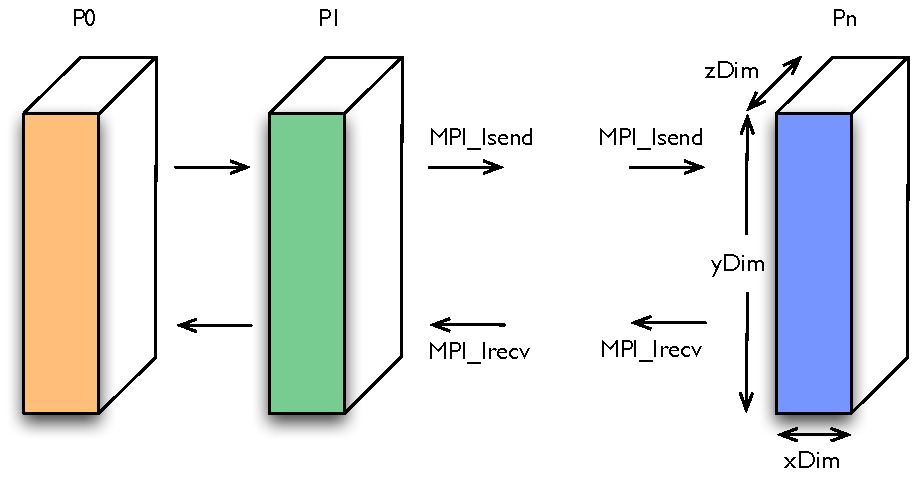
\includegraphics[width=\textwidth]{images/mpi_decomp}}
%\begin{center}
%Model bulk-synchronous Numerical Simulation
%\end{center}
%\end{frame}

%\begin{frame}
%\frametitle{Model Bulk-Synchronous MPI+OpenMP Application Code}
%\begin{center}
%\begin{figure}[ht]
%\lstinputlisting{/Users/kale2/hybridscheduling/listings/omp-static.c}
%\end{figure}
%\end{center}
%\end{frame}



\comments{
\begin{frame}
\frametitle{Model Bulk-synchronous code }
\lstinputlisting{/Users/kale2/hybridscheduling/listings/mpi-bulk-synch.c}
\begin{center}
\includegraphics[scale=0.65]{/Users/kale2/hybridscheduling/images/appTimestep}
\end{center}
\end{frame}

\begin{frame}
\frametitle{Model Bulk-synchronous Hybrid MPI+OpenMP code }
\lstinputlisting{/Users/kale2/hybridscheduling/listings/omp-static.c}
\begin{center}
\includegraphics[scale=0.45]{/Users/kale2/hybridscheduling/images/emptySchedImage}
\end{center}
\end{frame}

\begin{frame}
\frametitle{Model Hybrid MPI+OpenMP Code}
\visible<1->{\lstinputlisting{/Users/kale2/hybridscheduling/listings/omp-static.c}}
\visible<2->{\includegraphics[scale=0.35]{/Users/kale2/hybridscheduling/images/legend-appTimestep}}
\end{frame}

\begin{frame}
\frametitle{Conceptual Diagram of Timestep }
%\lstinputlisting{/Users/kale2/hybridscheduling/listings/omp-static.c}
\includegraphics[scale=0.35]{/Users/kale2/hybridscheduling/images/legend-appTimestep}
\begin{center}
\includegraphics[scale=0.45]{/Users/kale2/hybridscheduling/images/appTimestep}
\end{center}
%\includegraphics[scale=0.35]{/Users/kale2/hybridscheduling/images/legend-twocol}
%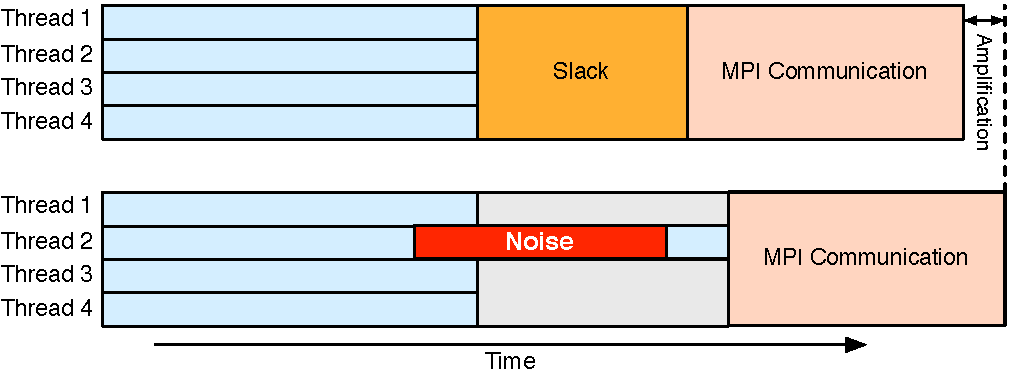
\includegraphics[scale=0.45]{/Users/kale2/hybridscheduling/images/static-schedule}
\begin{center}
\includegraphics[scale=0.45]{/Users/kale2/hybridscheduling/images/emptySchedImage}
\end{center}
\end{frame}

\begin{frame}
\frametitle{Amplification}
\includegraphics[scale=0.35]{/Users/kale2/hybridscheduling/images/legend-static}
\begin{center}
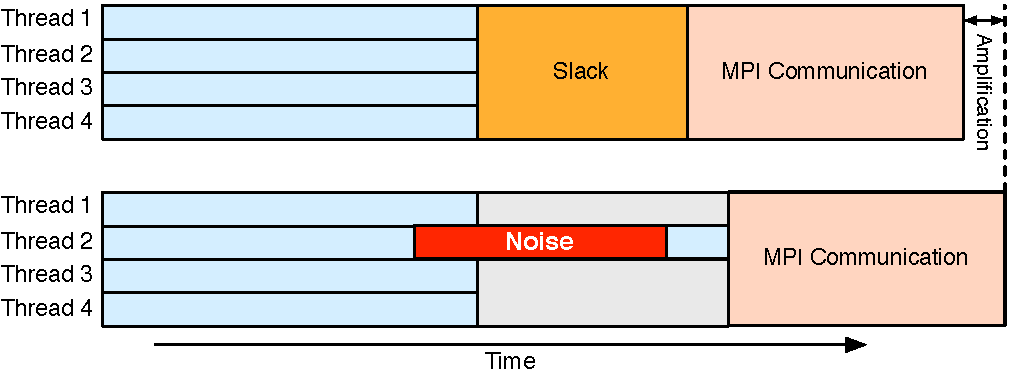
\includegraphics[scale=0.45]{/Users/kale2/hybridscheduling/images/static-schedule}
\end{center}
\begin{center}
\includegraphics[scale=0.45]{/Users/kale2/hybridscheduling/images/emptySchedImage}
\end{center}
\end{frame}


\begin{frame}
\frametitle{Assumption: Application is load balanced }
\begin{itemize}
\item \small Assume that problem is load balanced across MPI processes.
\item \small If problem isn't load balanced across MPI processes, then some other ``classical'' load balancer takes care of it.
\end{itemize}
\end{frame}

%\begin{frame}
%\frametitle{Localized Coordinated+Uncoordinated Load Imbalance}
%\begin{itemize}
%\item \small Assume that problem is load balanced across MPI processes.
%\item \small If problem isn't load balanced across MPI processes, then some other ``classical'' load balancer takes care of it.
%\item \small Imbalance stays within-node, or within racks
%\end{itemize}
%\end{frame}


\begin{frame}
\frametitle{Uncoordinated Transient Load Imbalance}
\begin{itemize}
\item \small If in iteration 304, if node 7 experiences excess work, it is not necessary that other nodes experience excess work in the same iteration.
\item \small If core 3 of node 7 has excess work, it does not mean core 3 of node 19 has excess work.
\item \small No pattern of load imbalances across MPI processes(show across space).
\end{itemize}
\end{frame}

\begin{frame}
\frametitle{Traditional load balancers are of no help }
\begin{enumerate}
\item \small Traditional load balancers,e.g. Measurement-based load balancer, handle load imbalances that persist over time
\item \small Here, no patterns of load imbalance across time, so can't use measurement-based load balancing.
\item \small Load imbalance happens with a certain probability on a node.
\item \small On each timestep, load imbalance happens with higher probability as we scale (as probabilities add up).
\item \small The probability of load imbalance occurring in one timestep increases as we scale (as probabilities add up).
\end{enumerate}
\end{frame}

\begin{frame}
\frametitle{Localized Uncoordinated Transient Load Imbalance}
\begin{itemize}

\end{itemize}
\end{frame}

}


%1. TO DO: do excel simulation for noise amplification curves for delta, p and T.  Also, consider modified delta after mitigation .

%%2. TO DO :  do experimentation for check asynchronous collectives

%\begin{frame}
%\frametitle{Why not asynchronous collectives?}
%\begin{itemize}
%\item suppose you have fraction f of work(from the next timestep/iteration) that you can do before results of the collective are available . What is the impact on amplification?
%\item
%\end{itemize}
%\end{frame}

\comments{

\begin{frame}
\frametitle{ What is the right amount of dynamic scheduling to use?(theory) }
\begin{itemize}
\item theoretical analysis
\end{itemize}
\end{frame}


% add in where ROSE comes in, and source to source comes in.
% put in MPI application specifics and code
% put in impact of compiler (icc vs. gcc)

\begin{frame}
\frametitle{Resilient Scheduling Strategy Applied to Model Synchronous MPI+OpenMP Code}
\lstinputlisting{/Users/kale2/hybridscheduling/listings/omp-static.c}
\lstinputlisting{/Users/kale2/hybridscheduling/listings/omp-hybrid.c}
\end{frame}

\begin{frame}
\frametitle{High-level Software Design}
\includegraphics[width=\textwidth]{/Users/kale2/hybridScheduling/images/architecture}
\end{frame}

\begin{frame}
\frametitle{Scaling with Resilient Scheduling}
\begin{figure}[h]
\label{fig:app-scaling-hera}
\begin{center}
\includegraphics[width=\columnwidth]{/Users/kale2/hybridscheduling/plots/app-scaling-hera}
\end{center}
\begin{center}
\tiny Percent speedup of callsite strategy over baseline stat. sched. on sierra.
\end{center}
\end{figure}

\begin{figure}[h]
\label{fig:app-scaling-rzuseq}
\begin{center}
%\includegraphics[width=\columnwidth]{/Users/kale2/hybridscheduling/plots/app-scaling-rzuseq}
\includegraphics[width=\columnwidth]{plots/app-scaling-rzuseq}
\end{center}
\begin{center}
\tiny Percent speedup of callsite strategy over baseline stat. sched. on rzuseq.
\end{center}
\end{figure}

%\begin{itemize}
%\small \item \tiny \textit{Static-Hybrid} gives moderate perf gains, as can be seen in figure~\ref{fig:app-scaling-hera}.
%\item \tiny Resilient-Callpath gives best perf. gain of all slack-conscious strategies, as seen in figure~\ref{fig:app-scaling-hera}.
%\item \tiny Resilient-Coll and Resilient-Naive give limited perf gains, likely due to
%  mispredictions, which outweigh the overhead of the prediction.
%\item \tiny As seen in figure ~\ref{fig:app-scaling-rzuseq}, the \textit{Resilient-Callpath} method does not cause large degradations, showing
%that using the methodology does not interfere greatly with the performance of the application.
%\end{itemize}
\end{frame}
}
